\documentclass[11pt]{article}

% --- arXiv-safe preamble: mainstream packages only ---
\usepackage[utf8]{inputenc}
\usepackage[T1]{fontenc}
\usepackage{lmodern}
\usepackage{amsmath,amssymb}
\usepackage{booktabs}
\usepackage{array}
\usepackage{geometry}
\usepackage{microtype}
\usepackage{graphicx}
\usepackage[hidelinks]{hyperref}
\geometry{margin=1in}

\newcommand{\V}{\textit{V}}

\title{\textbf{Wide but Shallow}\\[2pt]
\large Technical-Interview Problems Are Four Ideas in Many Costumes\\[4pt]
\normalsize\itshape and company-specific preparation is mostly a myth}

\author{Conor Garvey Gelvin\\ \texttt{gelvin@outlook.com}}
\date{Data snapshot: June 2026 \quad$\cdot$\quad Draft}

\begin{document}
\maketitle

\begin{abstract}
Interview-prep advice rests on two claims: that different companies test different skills, and that you must
memorize dozens of separate problem ``patterns.'' We test both against how often each problem appears among
seven major technology firms' most-asked lists (769 distinct problems), and both mostly fail. The roughly
twenty ``patterns'' you are told to learn are really \textbf{four underlying ideas}: a single left-to-right
pass (a \emph{fold}), divide-and-solve recursion (dynamic programming), spreading information across a graph
until it settles, and binary search. The single pass is the most common, and many tricks taught as
unrelated---prefix sums, the XOR trick, a hash ``seen set,'' reversing a list, the sliding window---are the
\emph{same} pass; they differ only in what running value they carry. To keep our labels honest we did not
just hand-sort the problems: we re-checked a random sample of 100 with the Lean proof assistant, which
verifies each claim mechanically. \textbf{76 of the 100} carry a machine-checked, \emph{problem-specific}
certificate (two more carry only a weaker structural one and are not counted). Separately, the seven firms
ask almost the same mix of the four ideas: on a standard $0$-to-$1$ scale of how differently they ask
(bias-corrected Cram\'er's \V, where $0$ is identical), they score just $0.091$, above the $0.065$ noise
floor but far below ``moderate''---small enough that six of the seven are statistically indistinguishable,
and only Uber stands out (it leans on graph problems). We describe which problems are \emph{commonly asked},
not how hard they are or whether company-specific drilling pays off. In short: interview problems are
\emph{wide on the surface but shallow underneath}, and essentially one shared syllabus covers nearly every
company. All derived data and proofs are released; the raw scrape is withheld per the platform's terms.
\end{abstract}

\section{Two myths}
\label{sec:intro}

Two beliefs dominate interview preparation. The first is \emph{company specificity}: that Google, Meta,
Amazon and their peers test different skills, so you should prepare differently for each. The second is
\emph{pattern proliferation}: that the field is a long list of loosely related tricks---sliding window,
monotonic stack, union--find, prefix sums, and so on---each learned separately, as popular pattern
catalogues present them~\cite{prashad}. Both are widely repeated and, as far as we can tell, never tested.

We test them, and then ask what underlying \emph{structure} explains the answer. The short version: the
``fifty patterns'' you are told to memorize are a handful of ideas in different disguises, and the seven
companies ask nearly the same things. To keep our labels honest we do not hand-sort the problems and stop
there---we use a proof assistant to check, problem by problem, that the idea we assign really does solve the
problem (and, for several showcase examples, that the standard solution is fully correct).

\section{Data and method}
\label{sec:data}

For seven firms (Amazon, Apple, Bloomberg, Google, Meta, Microsoft, Uber) we scraped a public
interview-prep platform for how often each problem appears among that firm's \emph{most-asked} problems
(the platform exposes a top-200 list per firm and recency window, so rarely-asked problems are truncated;
we note this where it matters). Across firms this covers 769 distinct problems, broken down by recency. The
platform tags each one with a \emph{surface family} (``sliding window,'' ``monotonic stack,'' ``dynamic
programming,'' and so on), which we consolidate into about twenty broad families.

A fixed rule, written down in advance (Appendix~\ref{sec:rule}), maps each family to one of our four
underlying \emph{ideas} (formally, \emph{recursion schemes})---a coarser label based on the \emph{shape} of
the standard solution rather than its textbook name (Table~\ref{tab:schemes})---or to a leftover ``tail'' for
problems that fit no single idea. We
ask two separate questions and keep them apart: \emph{coverage}---what fraction of problems the four ideas
explain---measured on a random sample of distinct problems (Section~\ref{sec:lean}); and the \emph{company}
comparison---do firms ask different mixes?---measured by weighting each idea by how often it is asked
(Section~\ref{sec:result}). The company comparison groups by the four ideas, with the finer twenty-family
view reported alongside as a robustness check; all difference measures are bias-corrected~\cite{bergsma13}
and reported with uncertainty.

\section{Result: four ideas, not fifty}
\label{sec:result}

\begin{table}[t]
\centering
\small
\begin{tabular}{@{}>{\raggedright\arraybackslash}p{2.3cm}>{\raggedright\arraybackslash}p{5.0cm}rrl@{}}
\toprule
Recursion scheme & textbook families it subsumes & assigned & certified & Lean witness \\
\midrule
streaming fold & two-pointers, sliding-window, monotonic-stack, hashing, prefix-sum, linked-list, bit-XOR, string-scan & 29 & 29 & \texttt{IsFold} \\
recursive decomposition (DP) & dynamic programming, backtracking, tree & 25 & 24 & catamorphism \\
graph relaxation & BFS/DFS, Dijkstra, Bellman--Ford, topo-sort, union--find & 15 & 15 & least fixpoint \\
bisection & binary search (monotone predicate) & 9 & 8 & monotone threshold \\
\midrule
\textbf{in a scheme} & & \textbf{78} & \textbf{76} & \\
not a scheme & design, simulation, heaps, number theory, string matching, $\dots$ & 22 & --- & --- \\
\bottomrule
\end{tabular}
\caption{The roughly twenty surface families collapse onto four recursion schemes. On a uniform random
sample of 100 distinct problems: ``assigned'' is how many the fixed rule (Appendix~\ref{sec:rule}) places in
each scheme; ``certified'' is how many additionally carry a Lean certificate whose correctness proof is
\emph{problem-specific} (Section~\ref{sec:lean}). 76 of 100 are certified (95\% Wilson interval
$[0.67,0.83]$). The ``Lean witness'' is the formal predicate each scheme is checked against
(\emph{catamorphism}: a fold over a tree-shaped structure; \emph{least fixpoint}: the limit of one-step
graph relaxation). \emph{Every} assigned problem carries a formal certificate that builds (78 of 78); 76 of
those additionally prove a problem-specific correctness property. The two that do not---Burst Balloons (its
interval-DP \emph{optimality}) and Block Placement Queries (its segment-tree query structure)---carry only a
structural certificate, as a faithful proof exceeds one self-contained file; we conservatively leave them
uncounted. Certificate strength among the 76 still varies: full correctness for the flagship folds of
Section~\ref{sec:lean}, a one-directional property (e.g.\ soundness, or existence) otherwise.}
\label{tab:schemes}
\end{table}

\paragraph{Wide surface.} The surface taxonomy really is spread out: no one or two families dominate (it
takes six of the $\sim$20 to cover even half of asked problems; Gini $0.30$ over distinct problems). By the
usual measure, interview preparation \emph{looks} like a long, flat list. This is the breadth the prep
industry sells.

\paragraph{Shallow root.} But that breadth is mostly repackaging. When we sort the same problems by the
\emph{shape} of their standard solution, the four ideas cover 76 of 100 sampled problems
(Table~\ref{tab:schemes}; 95\% confidence interval $[67\%,83\%]$), and the single left-to-right pass is the
most common of them. Tricks memorized as unrelated---prefix sums, the XOR trick, a hash ``seen set,''
reversing a list, matching parentheses with a stack, the sliding window---are the \emph{same} pass; they
differ only in what running value they carry. The variety is in the bookkeeping, not in the computation.

\paragraph{One shared syllabus.} The same data dissolve the company myth. We score how differently the firms
ask on a standard $0$-to-$1$ scale (bias-corrected Cram\'er's \V~\cite{cramer46,bergsma13}, where $0$ means
identical and the usual cutoffs call $0.1$ ``small'' and $0.3$ ``moderate''). Across the four ideas the firms
score just $\V = 0.091$ (95\% confidence interval $[0.06,0.12]$)---small, with the whole interval well below
``moderate,'' so the difference is genuinely bounded, not merely undetected. We headline the four-idea
grouping because its score clears the noise floor that finite samples generate by chance ($0.091$ versus a
null of $0.065$); at the finer twenty-family level the score is \emph{below} its own floor ($0.064$ versus
$0.116$), i.e.\ statistically indistinguishable from identical---so the finer view, if anything, makes the
firms look more alike, not less. Comparing firms two at a time, the only real
differences all involve \textbf{Uber}, which asks more graph problems and fewer single-pass ones (its largest
gap, versus Google, is still only ``small''; Figure~\ref{fig:resid}); \textbf{the other six firms are
statistically indistinguishable}. One caveat: we compare the \emph{mix of problem types}, not how hard the
problems are or whether drilling for a specific company helps---our data cannot measure those. Within that
scope, there is essentially one interview syllabus, and preparing differently per company is, for most firms,
wasted effort.

\begin{figure}[t]
\centering
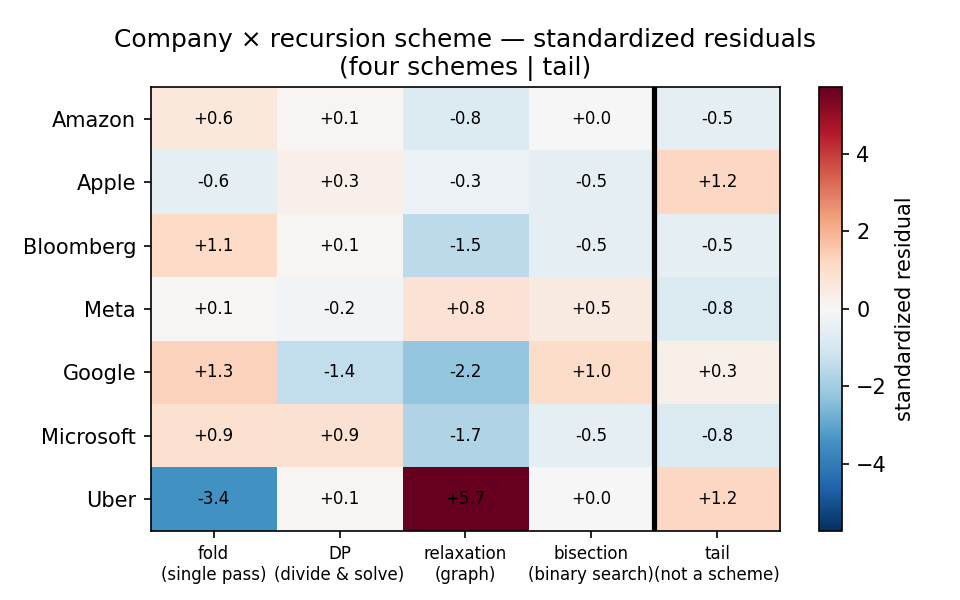
\includegraphics[width=0.78\linewidth]{figs/residual_scheme.png}
\caption{How much each firm over- or under-asks each idea, relative to the shared average (standardized
residuals; red = more than expected, blue = less). Only Uber stands out---it asks far more graph problems
($+5.7$) and far fewer single-pass ones ($-3.4$)---while the other six rows are muted (all within about
$\pm2$). This is the picture behind the small overall difference (\V$\,=0.091$): one shared syllabus, with
Uber the lone exception.}
\label{fig:resid}
\end{figure}

\section{Machine-checking the classification}
\label{sec:lean}

A classification is only as trustworthy as its labels. The usual check---a second human rater---only tells
you whether two people read a label the same way. We do something stronger: we check the labels with a
\emph{proof assistant}, a tool that mechanically verifies mathematical claims. Working in
Lean~4~\cite{lean4} with its library Mathlib~\cite{mathlib20}, we write each of the four ideas as a precise
test on programs (for example, ``this function is a single left-to-right pass''), and for a random sample of
100 problems we prove two things. First, \textbf{the idea fits} (\texttt{cls}): we exhibit the standard
solution in the form of its assigned idea (the scheme predicate holds of a concrete solution). Second,
\textbf{the solution is sound} (\texttt{corr}): that solution satisfies a verified correctness property
(often one direction of the guarantee, e.g.\ ``everything it reports is valid''). A problem counts only
when both proofs go through with no gaps (Lean flags unfinished proofs; there are none), using only Lean's
standard logical axioms, \emph{and} the correctness property is \textbf{problem-specific}---it refers to the
concrete problem (this grid, these subarrays, this sorted array), not to an abstract relation or predicate
that every problem in the scheme would satisfy equally. This last condition is the load-bearing one: a
certificate stated over a free relation certifies the \emph{scheme}, not the \emph{problem}, and we
mechanically exclude such certificates from the count (the gate is part of the released build script). Two
problems survive only as scheme-generic or structural certificates---Burst Balloons and Block Placement
Queries, whose genuine guarantees (interval-DP optimality; a segment-tree query invariant) need machinery
beyond a single self-contained file---and we do not count them, leaving 76.

\textbf{What this does and does not show.} The two proofs cover an example of the idea and a working
solution---but we do not separately prove that those two are the \emph{same} program. So a certificate says
``this problem really is solvable by idea $S$, and we have a verified-correct solution,'' not ``the
platform's exact accepted code is literally a single pass.'' That is weaker than proving the two coincide
(which we flag in Section~\ref{sec:threats}), but far stronger than an unchecked label: a concrete solution
in the scheme's form exists, and a solution is proven sound against the specific problem.

\textbf{The strongest examples.} For a few textbook cases we close that gap completely: the standard solution
\emph{is} the single pass, and we prove it correct as such. The cleanest is Kadane's algorithm for Maximum
Subarray---the answer is literally one pass carrying a running pair, and we prove it returns exactly the
largest possible subarray sum (both that the value is achievable \emph{and} that nothing beats it). Product
Except Self is a running-products pass with its key identity proven, and Single Number is the XOR pass proven
to return the lone unpaired value. For these the certificate is the strong form---``the code \emph{is} this
pass, and it is correct''---which is what the general procedure approximates for the rest.

The result is one reproducible number: 76 of 100, with a 95\% confidence interval of $[67\%,83\%]$ (a Wilson
interval, standard for a proportion). The certified list ships with the sample, so the count re-derives
directly. Two notes on honesty. The sample is the certification \emph{target}, not a test set: we attempt a
problem-specific certificate for every sampled in-scheme problem and count only those that go through, so
anything we cannot formalize to that standard---the two structural certificates above, and every tail
problem---stays uncounted. The count is therefore a coverage figure that errs low, not an error rate. We
also do not re-prove the deep theory behind the ideas---that shortest paths and dynamic programming are
formally well-founded is already established~\cite{afp_dijkstra,afp_kleene,lehmann77,afp_dp}, which we cite
rather than redo.

\section{Related work}
\label{sec:related}

Two literatures bracket this paper. On the \emph{empirical} side, interview preparation is organized by
pattern catalogues~\cite{prashad} that enumerate surface families; we are not aware of prior work that tests
whether those families are generatively distinct, or whether firms differ in the mix they ask. On the
\emph{structural} side, the observation that wide families of programs are instances of a few recursion
schemes is the Bird--Meertens tradition of program calculation~\cite{bird-demoor} and its formal-methods
descendants: associative aggregation over a sliding window is a verified fold~\cite{afp_sliding}, dynamic
programming is verified memoized recursion~\cite{afp_dp}, and shortest paths are a least fixpoint over a
semiring~\cite{afp_dijkstra,afp_kleene,lehmann77}; verified-algorithms textbooks now develop these schemes end
to end~\cite{fav_book,nipkow_survey}. The four-scheme decomposition itself is therefore not new---it is the
classical Bird--Meertens repertoire. Our contribution is to connect that structural lens to the
\emph{empirical} distribution of interview problems (the company-comparison test), and to machine-check the
scheme assignment per problem rather than assert it.

\section{Threats to validity}
\label{sec:threats}

\textbf{One platform.} The frequencies come from a single prep platform and may reflect its own collection
process as much as what employers truly ask; we describe \emph{commonly-asked} problems, not any firm's
private bar. \textbf{Top-200 cap.} Each firm's frequencies are its \emph{most-asked} top-200 list per recency
window, not the full distribution, so the rare tail is truncated; the company comparison is over the heads of
the distributions, where the data are densest. \textbf{Borrowed labels.} The family-to-idea rule is ours, but
the surface-family tags it starts from are the platform's---single-source and un-audited---so the ``wide
surface'' count inherits whatever splits that taxonomy chose. \textbf{The model is a choice.} The proof checks
that a problem \emph{can} be solved by an idea; it cannot certify that ``which idea it is'' is the right way to
describe what an interview tests. That a problem ``is a single pass'' is our modeling choice---the proof
confirms the model holds, not that it is the only sensible one. \textbf{Idea and solution proven separately.}
As in Section~\ref{sec:lean}, we prove the idea fits and, separately, that a solution is sound; proving the two
are the same program is done only for the showcase examples and is otherwise future work. \textbf{An estimate,
not a floor.} 76\% is a sample estimate; the confidence interval $[67\%,83\%]$, not the point value, is the
honest summary. The procedure undercounts in two ways---a problem we cannot formalize stays uncounted, and the
fixed rule conservatively routes borderline scan-shaped or binary-search-shaped families (e.g.\ parts of
``greedy'' and ``simulation'') into the tail rather than into \texttt{fold}/\texttt{bisection}---so 76\% is if
anything a lower bound on how many problems reduce to the four ideas. But ``conservative'' describes the
measurement, not a guarantee about all problems. \textbf{Window dependence.} The company difference is not
constant across recency windows: the bias-corrected \V\ ranges from below its noise floor in the short windows
up to $0.125$ in the six-month window (still ``small''), so ``one shared syllabus'' is a statement about the
pooled data, not every slice. \textbf{Two separate questions.} Coverage counts each distinct problem once; the
company comparison weights by how often a problem is asked. Both matter to a candidate, and we keep them
apart. \textbf{Shallow is not easy.} ``Same idea'' does not mean ``same difficulty''---two single-pass
problems can differ hugely in how hard the running value is to find. We claim shallow \emph{structure}, not
that the problems are easy.

\section{Conclusion}

Interview problems are wide on the surface but shallow underneath. The roughly twenty ``patterns'' are four
ideas in different disguises: on a random sample, 76 of 100 problems carry a machine-checked, problem-specific
certificate that the assigned idea really solves them and that a standard solution is sound (95\% confidence
interval $[67\%,83\%]$; the single left-to-right pass is the most common). And the seven firms ask essentially one
shared syllabus. For a candidate, the takeaway is blunt: learn the four ideas deeply rather than fifty
patterns shallowly, and prepare for ``technical interviews,'' not for any one company.

\section*{Reproducibility and AI-use disclosure}

All derived statistics, the family-to-idea rule (released as a standalone table, fixed in advance so anyone
can check the categories were not tuned to fit the sample), the sampling seed, the certified list (from which
the 76/100 re-derives), and the complete Lean development are released. The problem-specific gate that
separates the 76 counted certificates from the 2 merely-structural ones is itself a released, mechanical
script, so the headline count is reproducible rather than a matter of our judgement. The raw per-company
frequency tables are withheld under the platform's terms, so the headline numbers reproduce from the released
derived data even though the scrape itself is not redistributed. The proofs build with \texttt{lake build}
with no gaps; the ``standard axioms'' claim is checkable, not merely asserted, by running \texttt{\#print
axioms} on the main theorems. This paper was written by one human author with substantial AI assistance for drafting,
statistical code, and the formalization; all claims, numbers, and proofs were checked by the author, and the
machine-checked results are independently verifiable by re-running the proofs. We say so plainly: the paper's
central claims stand or fall on the released data and the proofs, not on how it was written.

\begin{thebibliography}{99}
\bibitem{prashad} S.~Prashad. LeetCode Patterns. \url{https://seanprashad.com/leetcode-patterns/}, 2020.
\bibitem{cramer46} H.~Cram\'er. \emph{Mathematical Methods of Statistics}. Princeton
University Press, 1946.
\bibitem{bergsma13} W.~Bergsma. A bias-correction for Cram\'er's \emph{V} and Tschuprow's
\emph{T}. \emph{Journal of the Korean Statistical Society}, 42(3):323--328, 2013.
\bibitem{lean4} L.~de Moura and S.~Ullrich. The Lean~4 theorem prover and programming
language. In \emph{Automated Deduction (CADE-28)}, 2021.
\bibitem{mathlib20} The mathlib Community. The Lean mathematical library. In \emph{Proc.\
9th ACM SIGPLAN Int.\ Conf.\ on Certified Programs and Proofs (CPP)}, 367--381, 2020.
\bibitem{afp_dijkstra} B.~Nordhoff and P.~Lammich. Dijkstra's shortest path algorithm.
\emph{Archive of Formal Proofs}, 2012.
\bibitem{afp_kleene} A.~Armstrong, G.~Struth, and T.~Weber. Kleene algebra.
\emph{Archive of Formal Proofs}, 2013.
\bibitem{lehmann77} D.~J. Lehmann. Algebraic structures for transitive closure.
\emph{Theoretical Computer Science}, 4(1):59--76, 1977.
\bibitem{afp_dp} S.~Wimmer, S.~Hu, and T.~Nipkow. Monadification, memoization and dynamic
programming. \emph{Archive of Formal Proofs}, 2018.
\bibitem{bird-demoor} R.~Bird and O.~de Moor. \emph{Algebra of Programming}. Prentice Hall, 1997.
\bibitem{afp_sliding} L.~Heimes, D.~Traytel, and J.~Schneider. Formalization of an algorithm for
greedily computing associative aggregations on sliding windows. \emph{Archive of Formal Proofs}, 2020.
\bibitem{fav_book} T.~Nipkow, J.~Blanchette, M.~Eberl, A.~G\'omez-Londo\~no, P.~Lammich,
C.~Sternagel, S.~Wimmer, and B.~Zhan. \emph{Functional Algorithms, Verified!} 2021.
\url{https://functional-algorithms-verified.org}.
\bibitem{nipkow_survey} T.~Nipkow, M.~Eberl, and M.~P.~L.~Haslbeck. Verified textbook algorithms:
A biased survey. In \emph{Automated Technology for Verification and Analysis (ATVA)}, 2020.
\end{thebibliography}

\appendix
\section{Family-to-scheme assignment rule}
\label{sec:rule}

Each surface family is mapped to the scheme matching the \emph{shape of its canonical accepted solution}: a
single left-to-right pass carrying one accumulator $\to$ \emph{streaming fold}; a recurrence that
decomposes a structure into sub-results $\to$ \emph{recursive decomposition (DP)}; iterative improvement
toward a fixed point over a graph $\to$ \emph{graph relaxation}; a monotone predicate located by halving
$\to$ \emph{bisection}; anything else (bespoke data structures, simulation, ad-hoc number theory, string
matching) $\to$ \emph{tail}. The rule is applied to the family, not tuned per problem; the per-problem Lean
checks (Section~\ref{sec:lean}) then test whether the assigned scheme actually solves each sampled problem.

\end{document}
